%!TEX ROOT = main.tex

\section{Final Project}

The purpose of the final project is to implement an efficient agent that can play and win Quarto. Quarto is a multi-player game where 2 players take turns placing pieces on a 4x4 board. The first player to place a piece that satisfies a winning condition wins the game. In my version of Quarto, I consider it to be a two-player game where my agent plays against a random opponent.

\subsection{Acknowledgements}

Throughout this project, I have discussed with Diego Gasco (s296762). We started the project by discussing ideas for strategies.

\begin{itemize}
    \item After I tried to get a working Deep Q-Network and realised that it wasn't converging in reasonable time, we discussed the possibility of using some tree search algorithm. It was Diego who suggested MCTS.
    \item When realising that MCTS can be quite slow towards the end of the game, I suggested building a hybrid QL-MCTS player that would use a base Q-table to remember the best moves so the quadratically complex tree wouldn't need to store so many nodes.
    \item We later built a hardcoded agent using different rules and realised that it performed very well, and was quick to make a move.
    \item We then decided to combine everything we did into a hybrid agent that would switch between strategies depending on the board score.
    \item Diego suggested a good scoring function. He also suggested that a genetic algorithm could be used for this.
    \item I suggested finding score thresholds to switch between strategies using a genetic algorithm.
\end{itemize}

While we follow the same hybrid strategy, our code is quite different, apart from a few shared utility functions.

The code for this project is available on \href{https://github.com/sidharrth2002/ci-quarto-sidharrth}{Github}.

\subsection{My Strategy For Solving the Problem}

\subsubsection{Step 1: Implement and Tune Multiple Search Algorithms}

The following algorithms are implemented and the \textbf{best performing ones are combined to create a final, hybrid agent that balances speed and efficiency}:

\begin{itemize}
    \item \textbf{Random}: This agent randomly selects positions and pieces on the board. In the spirit of true randomness, it does not take into account the current state of the board.
    \item \textbf{Parameterized Hardcoded Play}: This agent has a set of fixed rules, where it attempts to build a line of like pieces. Where it cannot, it attempts
    \item \textbf{Deep Q-Learning}: This agent uses a deep neural network to approximate the Q-function. It uses a replay buffer to store the experience tuples and uses a target network to stabilize the training process. The agent uses an epsilon-greedy policy to balance exploration and exploitation. The input to the linear network is a flatten list of 1x16 pieces based on the current board composition, while the input to the convolutional neural network is a 4x4x4 board composition.
    \item \textbf{Q-Learning (Temporal Difference Learning)}: This agent uses a Q-table to store the Q-values. It uses a replay buffer to store the experience tuples and uses a target network to stabilize the training process. The agent uses an epsilon-greedy policy to balance exploration and exploitation. A custom OpenAI Gym environment is created to make training easier.
    \item \textbf{Monte Carlo Tree Search}: This agent uses a Monte Carlo Tree Search algorithm to select the best move. It uses a UCB1 formula to select the best child node at each iteration.
    \item \textbf{QL-MCTS}: This algorithm uses a Q-table as it's base and uses a rolled out Monte Carlo Search Tree for a more efficient search. When a state cannot be found in the Q-table, the agent once again goes to the Monte Carlo Tree Search algorithm to find the best move.
\end{itemize}

The following algorithms failed, producing only a near-random win rate after several hours of training:

\begin{enumerate}
    \item \textbf{Pure Q-Learning}: This agent stores moves made in a Q-table and could not perform feasibly in a test environment even after hours of training, growing it's Q-table and implementing board symmetries.
    \item \textbf{Deep Q-Learning (Linear and Convolutional Neural Network)}: In this approach, I train a 4-layer deep neural network to predict the Q-values of a given state. Despite several hours of training and hyperparameter tuning (changing the number of layers, optimiser, learning rate), the agent could only reach a 60\% win rate in its best attempt. I also tried a convolutional neural network to feed the entire board composition as a 4x4x4 input (third dimension is the piece attribute), but training was far too slow.  \\ \\
    \textbf{Best Model Depth and Configuration}: 4-layer linear neural network of node sizes (24, 48, 96, 192), Huber Loss, Adam Optimiser, Learning Rate of 0.001

    \begin{equation*}
        L_{\delta}=
    \left\{\begin{matrix}
        \frac{1}{2}(y - \hat{y})^{2} & if \left | (y - \hat{y})  \right | < \delta\\
        \delta ((y - \hat{y}) - \frac1 2 \delta) & otherwise
    \end{matrix}\right.
    \end{equation*}

    \textbf{Best Results}: 55\% win rate after 1000 episodes of training \\ \\
    Training time was too slow and convergence could not be reached in a reasonable time. I had already spent multiple weeks on this approach to no fruition. If I had more computational resources, I would train this model for much longer to see if true convergence can be reached.
\end{enumerate}

\subsubsection{Step 2: Analysing the Algorithms}

The best performing algorithms were the hardcoded agent and Monte Carlo Tree Search, that produced high win rates (>80\%). However, important observations for each strategy are:

\begin{itemize}
    \item \textbf{Hardcoded Agent}: This agent is fast, but it is not efficient. It is only able to win the game if it is able to build a line of like pieces. If it cannot, it will return to a series of random moves that may/may not win the game.
    \item \textbf{Monte Carlo Tree Search}: MCTS rolls out and computes the reward from each board state but it is slow. It appears that it is not worth using at the start of the game, where a terminal state is quite distant from the current board position. Furthermore, a major problem with MCTS is the tree size, which grows exponentially with game progression. \textbf{This makes rolling out at each subsequent move slower than the previous rollout.} \\
\end{itemize}

Solution: Instead of keeping an extremely large tree, we record the result of each \textit{state, action} pair in a Q-table, updated using Temporal Difference Learning and the Bellman equation. On the off chance that a past board state is encountered, the Q-table can be used to find the best corresponding action, instead of having to iterate through the entire tree. I call this the \textbf{QL-MCTS} algorithm, with inspiration from Wang et al. (2018) approach to Monte-Carlo Q-Learning. QL-MCTS works by:

\begin{itemize}
    \item When training the Q-learning agent, use MCTS to find the best moves instead of using random in the epsilon-greedy policy.
    \item If the agent is called and a particular state-action combination is not present in the Q-table, go to MCTS to find the best move.
\end{itemize}

\subsubsection{Step 3: Implementing the Hybrid Agent}

Using the best performing algorithms, I created a hybrid agent that works in 3 phases. First, to get the game started, it will make random moves. After this, it will switch to a hardcoded strategy where it will attempt to computationally build lines of similar pieces. Finally, it will leverage the QL-MCTS algorithm to find the best moves and win the game. Since QL-MCTS is slow, it is kept as the final phase. This approach is shown in Figure \ref{fig:hybrid-agent}, and is a balance between speed and efficiency.

\begin{figure}
    \centering
    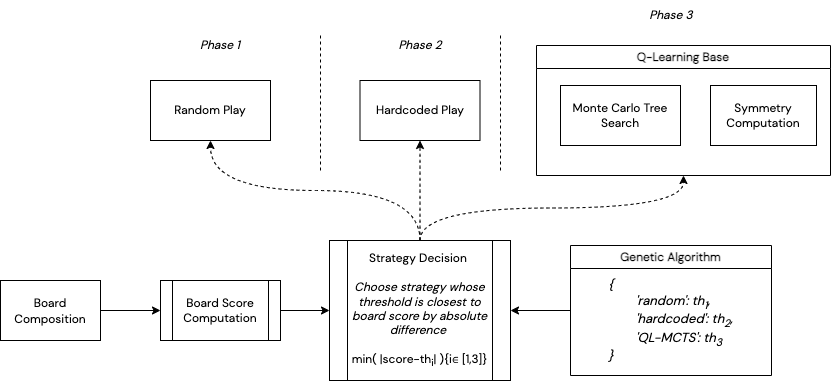
\includegraphics[width=0.9\textwidth]{images/methodology.drawio.png}
    \caption{Hybrid Agent}
    \label{fig:hybrid-agent}
\end{figure}

The main question is when to switch between the algorithms. The intuition is that the switch depends on the change of the board composition. We represent this numerically through a board score, that is essentially a sum of couplets and triplets.

\begin{equation*}
    couples + 2 * triplets
\end{equation*}

The range of values for scores $\in [0, 16]$. We try to generate score thresholds to switch between the 3 strategies using a genetic algorithm. An example of a genome is shown in Figure \ref{json-example}.

\begin{listing}
    \begin{minted}{json}
    {
        "random": 3,
        "hardcoded" : 5,
        "ql-mcts" : 8
    }
    \end{minted}
    \caption{Genome Example}
    \label{json-example}
    \end{listing}

We train the genetic algorithm for 1000 generations and a population size of 100, to find the best genome and submit these as the thresholds for the hybrid agent.

Once the final thresholds are found, we find the strategy whose threshold has the smallest absolute difference with the current board score. The minimisation formula is:

\begin{equation*}
    \text{strategy} = \min_{i=1}^{3} \left| \text{threshold}_i - \text{board score} \right|
\end{equation*}

\subsection{Results}

After several iterations of the genetic algorithm, the best genome thresholds were found to be:

\begin{minted}{json}
{
    'random': 2.090773081612301,
    'hardcoded': 3.790328881747581,
    'ql-mcts': 7.251997327518943
}
\end{minted}

It is clear that the algorithm prefers to use the QL-MCTS (essentially MCTS) strategy extensively, as it almost always guarantees a win regardless of whether it is playing first or second. Random is entirely probabilistic and hardcoded has better chances only when it's the first player.

Tournament results are shown in Table \ref{results}, where each player is played against a random player for 10 tournaments of 10 games each (10 x 10 = 100 games).

% put in table
\begin{table}[h]
    \centering
    \begin{tabular}{|c|c|c|}
        \hline
        \textbf{Strategy} & \textbf{Win Rate} & \textbf{Comments} \\ \hline
        DQN & 55\% & Convergence not reached \\ \hline
        QL-MCTS & 84\% & Slow, but can guarantee a win \\ \hline
        Hardcoded & 94\% & Fast \\ \hline
        Hybrid & 78\% & Heavily dependent on adjusting thresholds \\ \hline
    \end{tabular}
    \caption{Results computed based on 10 tournaments of 10 games each (10 x 10 = 100 games) against a random player}
    \label{results}
\end{table}

\subsection{Code of Hybrid Agent and Sub Players}

This subsection covers the code of the final hybrid agent and the sub players it calls periodically.

\subsubsection{Final Hybrid Player}

The final hybrid player's driver code is below. It uses a genetic algorithm to find the best thresholds for switching between the 3 strategies. It uses crossover and conditional mutations to find the best genome from a limited population size.

Furthermore, to reduce the search space, we enforce the constraint that the threshold for random < hardcoded < MCTS, with the the intuition that the slowest but most powerful algorithm should be used last.

\begin{mintedbox}{python}
'''
Genetic Algorithm for Quarto
'''
import sys
sys.path.insert(0, '..')

import tqdm
import random
import logging
import json
import itertools
from copy import deepcopy
from lib.players import Player, RandomPlayer
from quarto.objects import Quarto
from lib.scoring import score_board
from QLMCTS import QLearningPlayer
from Hardcoded.hardcoded import HardcodedPlayer

logging.basicConfig(level=logging.DEBUG)

class Genome:
    def __init__(self, thresholds, fitness):
        self.thresholds = thresholds
        self.fitness = fitness

    def set_fitness(self, fitness):
        self.fitness = fitness

    def set_thresholds(self, thresholds):
        self.thresholds = thresholds

    def toJSON(self):
        return {
            'thresholds': self.thresholds,
            'fitness': self.fitness
        }


class FinalPlayer(Player):
    '''
    Final player uses genetic algorithm to decide between:
    1. Hardcoded Strategy
    2. Random Strategy
    3. QL-MCTS
    '''

    def __init__(self, quarto: Quarto = None):
        if quarto is None:
            quarto = Quarto()
        super().__init__(quarto)
        self.ql_mcts = QLearningPlayer(quarto)
        self.hardcoded = HardcodedPlayer(quarto)
        self.random_player = RandomPlayer(quarto)
        self.BOARD_SIDE = 4
        self.GENOME_VAL_UPPER_BOUND = 16
        self.GENOME_VAL_LOWER_BOUND = 0
        self.thresholds = {
            'random': 1.090773081612301,
            'hardcoded': 2.790328881747581,
            'ql-mcts': 8.251997327518943
        }

    def generate_population(self, population_size):
        population = []
        for i in range(population_size):
            threshold = {}

            # make sure that value for random < hardcoded < ql-mcts
            threshold['random'] = random.random() * self.GENOME_VAL_UPPER_BOUND
            # find random number between random and 15
            threshold['hardcoded'] = threshold['random'] + \
                random.random() * (self.GENOME_VAL_UPPER_BOUND -
                                    threshold['random'])

            # find random number between hardcoded and 15
            threshold['ql-mcts'] = threshold['hardcoded'] + \
                random.random() * (self.GENOME_VAL_UPPER_BOUND -
                                    threshold['hardcoded'])

            assert threshold['random'] < threshold['hardcoded'] < threshold['ql-mcts']

            population.append(Genome(threshold, 0))
        return population

    def ensure_correct_ordering(self, new_thresholds):
        if new_thresholds['random'] > new_thresholds['hardcoded']:
            new_thresholds['random'], new_thresholds['hardcoded'] = new_thresholds['hardcoded'], new_thresholds['random']
        if new_thresholds['hardcoded'] > new_thresholds['ql-mcts']:
            new_thresholds['hardcoded'], new_thresholds['ql-mcts'] = new_thresholds['ql-mcts'], new_thresholds['hardcoded']
        if new_thresholds['random'] > new_thresholds['hardcoded']:
            new_thresholds['random'], new_thresholds['hardcoded'] = new_thresholds['hardcoded'], new_thresholds['random']
        return new_thresholds

    def crossover(self, genome1, genome2):
        new_thresholds = {}
        for key in genome1.thresholds:
            new_thresholds[key] = random.choice(
                [genome1.thresholds[key], genome2.thresholds[key]])

        # make sure that value for random < hardcoded < ql-mcts
        new_thresholds = self.ensure_correct_ordering(new_thresholds)
        return Genome(new_thresholds, 0)

    def mutate(self, genome):
        new_thresholds = {}
        genome_thresholds = genome.thresholds
        if random.random() < 0.4:
            new_thresholds['random'] = random.random() * \
                self.GENOME_VAL_UPPER_BOUND
            new_thresholds['hardcoded'] = random.choice(
                [genome_thresholds['random'], genome_thresholds['random'] +
                    random.random() * (self.GENOME_VAL_UPPER_BOUND - genome_thresholds['random'])])
            new_thresholds['ql-mcts'] = random.choice(
                [genome_thresholds['hardcoded'], genome_thresholds['hardcoded'] +
                    random.random() * (self.GENOME_VAL_UPPER_BOUND - genome_thresholds['hardcoded'])])

            new_thresholds = self.ensure_correct_ordering(new_thresholds)

            assert new_thresholds['random'] < new_thresholds['hardcoded'] < new_thresholds['ql-mcts']

            return Genome(new_thresholds, 0)
        return genome

    def evolve(self, num_generations=50):
        self.population_size = 50
        self.offspring_size = 10
        population = self.generate_population(self.population_size)

        pbar = tqdm.tqdm(total=num_generations)
        for gen in range(num_generations):
            pbar.update(1)
            logging.debug('Generation: {}'.format(gen))
            offpsring = []
            for i in range(self.offspring_size):
                parent1 = random.choice(population)
                parent2 = random.choice(population)
                child = self.crossover(parent1, parent2)
                child = self.mutate(child)
                child.fitness = self.play_game(child.thresholds, num_games=5)
                offpsring.append(child)
            population += offpsring
            population = sorted(
                population, key=lambda x: x.fitness, reverse=True)[:self.population_size]

            if gen % 5 == 0:
                logging.info('Saving population')
                with open('/Volumes/USB/population3.json', 'w') as f:
                    json.dump([genome.toJSON() for genome in population], f)

        # return the best genome's thresholds
        return population[0].thresholds

    def play_game(self, thresholds, num_games=10):
        wins = 0
        for game in range(num_games):
            logging.debug('Game: {}'.format(game))
            state = Quarto()
            player = 0

            # initialise with some random piece just to kickstart game
            state.set_selected_piece(self.random_player.choose_piece(state, 0))
            self.current_state = state

            # python passes by reference
            # agent will use the state, etc. to update the Q-table
            # this function also wipes the MCTS tree
            self.ql_mcts.clear_and_set_current_state(state)
            self.hardcoded = HardcodedPlayer(state)

            while True:
                # board score is the number of couples and triplets on the board
                # it is indicative of the change of the board state
                board_score = score_board(self.current_state)

                differences = [abs(board_score - thresholds[key])
                                for key in thresholds]
                min_diff = min(differences)
                index = differences.index(min_diff)
                key = list(thresholds.keys())[index]

                if player == 0:
                    if key == 'random':
                        logging.debug('random')
                        # play randomly
                        action = self.random_player.place_piece()
                        next_piece = self.random_player.choose_piece()
                        while self.current_state.check_if_move_valid(self.current_state.get_selected_piece(), action[0], action[1], next_piece) is False:
                            action = self.random_player.place_piece()
                            next_piece = self.random_player.choose_piece()
                        self.current_state.select(
                            self.current_state.get_selected_piece())
                        self.current_state.place(action[0], action[1])
                        self.current_state.set_selected_piece(next_piece)
                        self.current_state.switch_player()
                        player = 1 - player

                    elif key == 'hardcoded':
                        # play using hardcoded strategy
                        self.previous_state = deepcopy(self.current_state)
                        winning_piece, position = self.hardcoded.hardcoded_strategy_get_move()
                        next_piece = self.hardcoded.hardcoded_strategy_get_piece()
                        while self.current_state.check_if_move_valid(self.current_state.get_selected_piece(), position[0], position[1], next_piece) is False:
                            winning_piece, position = self.hardcoded.hardcoded_strategy_get_move(
                                self.current_state)
                            next_piece = self.hardcoded.hardcoded_strategy_get_piece(
                                self.current_state)
                        self.current_state.select(state.get_selected_piece())
                        self.current_state.place(position[0], position[1])
                        self.current_state.set_selected_piece(next_piece)
                        self.current_state.switch_player()
                        player = 1 - player

                    else:
                        # play using QL-MCTS
                        logging.debug('ql-mcts')
                        self.ql_mcts.previous_state = deepcopy(
                            self.current_state)
                        action = self.ql_mcts.get_action(self.current_state)
                        self.ql_mcts.previous_action = action
                        self.ql_mcts.current_state.select(
                            self.current_state.get_selected_piece())
                        self.ql_mcts.current_state.place(action[0], action[1])
                        self.ql_mcts.current_state.set_selected_piece(
                            action[2])
                        self.ql_mcts.current_state.switch_player()
                        player = 1 - player

                else:
                    # opponent is random
                    action = self.random_player.place_piece()
                    next_piece = self.random_player.choose_piece()
                    while self.current_state.check_if_move_valid(self.current_state.get_selected_piece(), action[0], action[1], next_piece) is False:
                        action = self.random_player.place_piece()
                        next_piece = self.random_player.choose_piece()
                        # WARNING: very often stuck in this loop
                    self.current_state.select(
                        self.current_state.get_selected_piece())
                    self.current_state.place(action[0], action[1])
                    self.current_state.set_selected_piece(next_piece)
                    self.current_state.switch_player()
                    player = 1 - player

                if self.current_state.check_is_game_over():
                    if 1 - self.current_state.check_winner() == 0:
                        print("Agent wins")
                        wins += 1
                        # TODO: QL reward update
                    else:
                        print("Player 2 wins")
                    break

        # fitness is the percentage of games won
        logging.debug(f"Win rate: {wins/num_games}")
        return wins/num_games

    def choose_piece(self):
        '''
        Choose piece for next player to place
        '''
        thresholds = self.thresholds

        # game is stored in parent
        self.current_state = self.get_game()

        board_score = score_board(self.current_state)

        differences = [abs(board_score - thresholds[key])
                        for key in thresholds]
        min_diff = min(differences)
        index = differences.index(min_diff)
        key = list(thresholds.keys())[index]

        # python passes by reference
        # agent will use the state, etc. to update the Q-table
        # this function also wipes the MCTS tree
        self.ql_mcts.clear_and_set_current_state(self.current_state)
        self.hardcoded = HardcodedPlayer(self.current_state)

        if key == 'random':
            logging.debug('random')
            # play randomly
            action = self.random_player.place_piece()
            next_piece = self.random_player.choose_piece()
            while self.current_state.check_if_move_valid(self.current_state.get_selected_piece(), action[0], action[1], next_piece) is False:
                action = self.random_player.place_piece()
                next_piece = self.random_player.choose_piece()
            return next_piece

        elif key == 'hardcoded':
            # play using hardcoded strategy
            logging.debug('hardcoded')
            self.previous_state = deepcopy(self.current_state)
            # winning_piece, position = self.hardcoded.hardcoded_strategy_get_move()
            next_piece = self.hardcoded.hardcoded_strategy_get_piece()
            # while self.current_state.check_if_move_valid(self.current_state.get_selected_piece(), position[0], position[1], next_piece) is False:
            #     winning_piece, position = self.hardcoded_strategy_get_move()
            #     next_piece = self.hardcoded_strategy_get_piece()
            return next_piece

        else:
            # play using QL-MCTS
            logging.debug('ql-mcts')
            self.ql_mcts.previous_state = deepcopy(
                self.current_state)
            action = self.ql_mcts.get_action(self.current_state)
            self.ql_mcts.previous_action = action
            self.ql_mcts.current_state.select(
                self.current_state.get_selected_piece())
            return action[2]

    def place_piece(self):
        # python passes by reference
        # agent will use the state, etc. to update the Q-table
        # this function also wipes the MCTS tree
        self.current_state = self.get_game()
        thresholds = self.thresholds

        # python passes by reference
        # agent will use the state, etc. to update the Q-table
        # this function also wipes the MCTS tree
        self.ql_mcts.clear_and_set_current_state(self.current_state)
        self.hardcoded = HardcodedPlayer(self.current_state)

        while True:
            # board score is the number of couples and triplets on the board
            # it is indicative of the change of the board state
            board_score = score_board(self.current_state)

            differences = [abs(board_score - thresholds[key])
                            for key in thresholds]
            min_diff = min(differences)
            index = differences.index(min_diff)
            key = list(thresholds.keys())[index]

            if key == 'random':
                logging.debug('random')
                # play randomly
                action = self.random_player.place_piece()
                next_piece = self.random_player.choose_piece()
                while self.current_state.check_if_move_valid(self.current_state.get_selected_piece(), action[0], action[1], next_piece) is False:
                    action = self.random_player.place_piece()
                    next_piece = self.random_player.choose_piece()
                return action[0], action[1]

            elif key == 'hardcoded':
                # play using hardcoded strategy
                logging.debug('hardcoded')
                self.previous_state = deepcopy(self.current_state)
                winning_piece, position = self.hardcoded_strategy_get_move()
                # next_piece = self.hardcoded_strategy_get_piece()
                # while self.current_state.check_if_move_valid(self.current_state.get_selected_piece(), position[0], position[1], next_piece) is False:
                #     winning_piece, position = self.hardcoded_strategy_get_move()
                #     next_piece = self.hardcoded_strategy_get_piece()
                return position[0], position[1]

            else:
                # play using QL-MCTS
                logging.debug('ql-mcts')
                self.ql_mcts.previous_state = deepcopy(
                    self.current_state)
                action = self.ql_mcts.get_action(self.current_state)
                self.ql_mcts.previous_action = action
                return action[0], action[1]

    def test_thresholds(self):
        thresholds = {'random': 10000,
                        'hardcoded': 3, 'ql-mcts': 1000}
        win_rate = self.play_game(thresholds, num_games=10)
        return win_rate

if __name__ == "__main__":
    final_player = FinalPlayer()
    # best_thresholds = final_player.evolve()
    # print(best_thresholds)

    average_win_rate = 0
    for i in range(10):
        win_rate = final_player.test_thresholds()
        average_win_rate += win_rate
    print(f"Average win rate: {average_win_rate}")
\end{mintedbox}

\subsubsection{Code for Hardcoded Strategy}

The strategy is outlined in this \href{https://scholarworks.umt.edu/cgi/viewcontent.cgi?article=1334&context=tme}{paper}. I implement it in Python below.

\begin{mintedbox}{python}
'''
Hardcoded player for Quarto
Follows risky strategy from paper:

"Developing Strategic and Mathematical Thinking via Game Play:
Programming to Investigate a Risky Strategy for Quarto"
by Peter Rowlett
'''
from copy import deepcopy
import itertools
import logging
import random

from lib.players import Player
from quarto.objects import Quarto

import sys
sys.path.insert(0, '..')

class HardcodedPlayer(Player):
    def __init__(self, quarto: Quarto = None):
        if quarto is None:
            quarto = Quarto()
        super().__init__(quarto)
        self.BOARD_SIDE = 4

    def check_if_winning_piece(self, state, piece):
        '''
        Simulate placing the piece on the board and check if the game is over
        '''

        for i in range(self.BOARD_SIDE):
            for j in range(self.BOARD_SIDE):
                if state.check_if_move_valid(piece, i, j, -100):
                    cloned_state = deepcopy(state)
                    cloned_state.select(piece)
                    cloned_state.place(i, j)

                    if cloned_state.check_is_game_over():
                        return True, [i, j]
        return False, None

    def hardcoded_strategy_get_piece(self):
        '''
        Returns a piece to be placed on the board
        '''
        state = self.get_game()

        possible_pieces = []
        for i in range(16):
            # check if the piece is a winning piece
            winning_piece, _ = self.check_if_winning_piece(state, i)
            if (not winning_piece) and (i not in list(itertools.chain.from_iterable(state.state_as_array()))) and (i != state.get_selected_piece()):
                possible_pieces.append(i)

        # if no pieces can be placed on board anymore (board full/game over), return -1
        if len(possible_pieces) == 0:
            # check if number of non-empty cells is 16
            if len([i for i in list(itertools.chain.from_iterable(state.state_as_array())) if i != -1]) == 16:
                return -1
            else:
                # there are possible pieces to be placed, but they are winning pieces/already in board
                on_board = list(itertools.chain.from_iterable(
                    state.state_as_array()))
                not_on_board = list(set(range(16)) - set(on_board))
                return random.choice(not_on_board)
        else:
            return random.choice(possible_pieces)

    def choose_piece(self):
        '''
        Returns a piece to be placed on the board
        '''
        return self.hardcoded_strategy_get_piece()

    def hardcoded_strategy_get_move(self, return_winning_piece_boolean=True):
        #  1. Play the piece handed over by the opponent:
        # (a) play a winning position if handed a winning piece;
        # (b) otherwise, play to build a line of like pieces if possible;
        # (c) otherwise, play randomly.
        # 2. Hand a piece to the opponent:
        # (a) avoid handing over a winning piece for your opponent to play;
        # (b) otherwise, choose randomly.

        state = self.get_game()

        board = state.state_as_array()
        selected_piece = state.get_selected_piece()
        # check if the selected piece is a winning piece
        winning_piece, position = self.check_if_winning_piece(
            state, selected_piece)
        if winning_piece:
            return selected_piece, position

        # check if the selected piece can be used to build a line of like pieces

        row_1 = [[0, 0], [0, 1], [0, 2], [0, 3]]
        # pieces in row 2
        row_2 = [[1, 0], [1, 1], [1, 2], [1, 3]]
        # pieces in row 3
        row_3 = [[2, 0], [2, 1], [2, 2], [2, 3]]
        # pieces in row 4
        row_4 = [[3, 0], [3, 1], [3, 2], [3, 3]]

        # pieces in column 1
        col_1 = [[0, 0], [1, 0], [2, 0], [3, 0]]
        # pieces in column 2
        col_2 = [[0, 1], [1, 1], [2, 1], [3, 1]]
        # pieces in column 3
        col_3 = [[0, 2], [1, 2], [2, 2], [3, 2]]
        # pieces in column 4
        col_4 = [[0, 3], [1, 3], [2, 3], [3, 3]]

        # pieces in diagonal 1
        diag_1 = [[0, 0], [1, 1], [2, 2], [3, 3]]
        # pieces in diagonal 2
        diag_2 = [[0, 3], [1, 2], [2, 1], [3, 0]]

        for line in [row_1, row_2, row_3, row_4, col_1, col_2, col_3, col_4, diag_1, diag_2]:
            # check if the selected piece can be used to build a line of like pieces
            characteristics = []
            empty_rows = []
            for el in line:
                x, y = el
                if board[x, y] != -1:
                    piece = board[x][y]
                    piece_char = state.get_piece_charachteristics(piece)
                    characteristics.append(
                        [piece_char.HIGH, piece_char.COLOURED, piece_char.SOLID, piece_char.SQUARE])
                else:
                    empty_rows.append(el)
                    characteristics.append([-1, -1, -1, -1])

            selected_piece_char = state.get_piece_charachteristics(
                selected_piece)
            selected_piece_char = [selected_piece_char.HIGH, selected_piece_char.COLOURED,
                                    selected_piece_char.SOLID, selected_piece_char.SQUARE]

            # check if characteristics has an empty row
            if [-1, -1, -1, -1] in characteristics:
                # count how many [-1, -1, -1, -1] are in characteristics
                empty_indexes = [i for i, x in enumerate(
                    characteristics) if x == [-1, -1, -1, -1]]

                empty_rows_count = characteristics.count([-1, -1, -1, -1])
                characteristics_copy = characteristics.copy()

                # proceeding to check couplets and see if they can build triplets
                # since 2 empty rows may be present and either could create a triplet, have to choose randomly later
                potential_moves = []

                for i, index in enumerate(empty_indexes):
                    position = empty_rows[i]
                    # insert the selected piece in the empty row
                    # empty_piece_index = characteristics.index(
                    #     [-1, -1, -1, -1])
                    characteristics = characteristics_copy.copy()
                    characteristics[index] = selected_piece_char

                    # check if any column has the same characteristics
                    col1 = [characteristics[0][0], characteristics[1][0],
                            characteristics[2][0], characteristics[3][0]]
                    col2 = [characteristics[0][1], characteristics[1][1],
                            characteristics[2][1], characteristics[3][1]]
                    col3 = [characteristics[0][2], characteristics[1][2],
                            characteristics[2][2], characteristics[3][2]]
                    col4 = [characteristics[0][3], characteristics[1][3],
                            characteristics[2][3], characteristics[3][3]]

                    col1 = [int(i) for i in col1]
                    col2 = [int(i) for i in col2]
                    col3 = [int(i) for i in col3]
                    col4 = [int(i) for i in col4]

                    # print(col1, col2, col3, col4)
                    def check_if_form_triplet(line):
                        # earlier we checked if we can complete a line
                        # here we check if we can form a triplet (one step away from completing a line)
                        return line.count(1) == 3 or line.count(0) == 3

                    # if len(set(col1)) == 1 or len(set(col2)) == 1 or len(set(col3)) == 1 or len(set(col4)) == 1:
                    if check_if_form_triplet(col1) or check_if_form_triplet(col2) or check_if_form_triplet(col3) or check_if_form_triplet(col4):
                        # this piece can be used to build a line of like pieces
                        logging.debug('playing to build a line of like pieces')
                        potential_moves.append(list(reversed(position)))

                    if len(potential_moves) >= 1:
                        if return_winning_piece_boolean:
                            # return True, list(reversed(empty_rows[-1]))
                            return True, random.choice(potential_moves)
                        else:
                            # move = list(reversed(empty_rows[-1]))
                            # move = list(reversed(position))
                            move = random.choice(potential_moves)
                            return move[0], move[1]

        # play randomly
        possible_moves = []
        for i in range(self.BOARD_SIDE):
            for j in range(self.BOARD_SIDE):
                for next_piece in range(16):
                    if state.check_if_move_valid(selected_piece, i, j, next_piece):
                        if return_winning_piece_boolean:
                            possible_moves.append([False, [i, j]])
                        else:
                            possible_moves.append([i, j])

        random_move = random.choice(possible_moves)
        return random_move[0], random_move[1]

        logging.debug(f"Selected piece: {selected_piece}")
        logging.debug(f"Board: {board}")
        logging.debug('no move found')

    def place_piece(self):
        '''
        Above function sometimes necessary to return additional information
        In game, first return value is not necessary
        '''
        return self.hardcoded_strategy_get_move(return_winning_piece_boolean=False)
\end{mintedbox}

\subsubsection{Monte Carlo Tree Search}

The implementation of MCTS and the rollout strategy is based on the minimal implementation \href{https://gist.github.com/qpwo/c538c6f73727e254fdc7fab81024f6e1}{here}.

\begin{mintedbox}{python}


from collections import defaultdict
import copy
import json
import logging
import math
import pickle
import random
from threading import Thread

import numpy as np
from lib.isomorphic import BoardTransforms
from lib.players import Player, RandomPlayer
from lib.utilities import Node, NodeDecoder, NodeEncoder

from quarto.objects import Quarto

logging.basicConfig(level=logging.INFO)


class MonteCarloTreeSearchEncoder(json.JSONEncoder):
    def default(self, obj):
        l = {
            'Q': {k.hash_state(): v for k, v in obj.Q.items()},
            'N': {k.hash_state(): v for k, v in obj.N.items()},

            # children is a dictionary of nodes
            'children': {k.hash_state(): [NodeEncoder().default(i) for i in v] for k, v in obj.children.items()},

            # 'children': [NodeEncoder().default(child) for child in obj.children],
            'epsilon': obj.epsilon,
        }
        return l

    def encode(self, obj):
        return super().encode(obj)

    def load_json(self, filename):
        with open(filename, 'r') as f:
            return json.load(f, cls=MonteCarloTreeSearchDecoder)


class MonteCarloTreeSearchDecoder(json.JSONDecoder):
    '''
    Recreate MonteCarloTreeSearch object from JSON
    '''

    def __init__(self, *args, **kwargs):
        json.JSONDecoder.__init__(
            self, object_hook=self.object_hook, *args, **kwargs)

    def object_hook(self, obj):
        children = {}

        for k, v in obj['children'].items():
            children[Node(hashed_state=k)] = [
                NodeDecoder().object_hook(node) for node in v]

        if 'Q' in obj:
            return MonteCarloTreeSearch(
                Q={Node(hashed_state=k): v for k, v in obj['Q'].items()},
                N={Node(hashed_state=k): v for k, v in obj['N'].items()},
                children=children,
                epsilon=obj['epsilon'],
            )
        return obj


def decode_tree(tree):
    return MonteCarloTreeSearchDecoder().object_hook(tree)


class MonteCarloTreeSearch(Player):
    '''
    Solve using Monte Carlo Tree Search
    '''

    def __init__(self, board=Quarto(), epsilon=0.1, max_depth=1000, Q=None, N=None, children=None):
        self.epsilon = epsilon
        self.max_depth = max_depth
        if Q is None:
            self.Q = defaultdict(int)
        else:
            self.Q = defaultdict(int, Q)
        if N is None:
            self.N = defaultdict(int)
        else:
            self.N = defaultdict(int, N)
        if children is None:
            self.children = dict()
        else:
            self.children = children
        self.MAX_PIECES = 16
        self.BOARD_SIDE = 4
        self.board = board
        self.random_factor = 0
        self.decisions = 0
        super().__init__(board)

    def set_board(self, board):
        self.board = board

    def choose(self, node):
        '''
        Choose best successor of node (move)
        Returns the board itself
        '''
        def score(n):
            logging.debug(f"Before reading in choose {n}")
            if self.N[n] == 0:
                return float('-inf')
            return self.Q[n] / self.N[n]

        # node is board Quarto
        node = Node(node)
        if node.is_terminal():
            logging.debug(node.board.state_as_array())
            raise RuntimeError("choose called on terminal node")

        # number of moves made in game
        self.decisions += 1

        for key in self.children:
            if key == node:
                return max(self.children[key], key=score).board

        self.random_factor += 1
        if node not in self.children:
            for key, value in self.children.items():
                if BoardTransforms().compare_boards(node.board.state_as_array(), key.board.state_as_array()):
                    if key in self.children:
                        print("found in symmetry")
                        return max(self.children[key], key=score).board

            # number of times have to resort to random
            rand_child = node.find_random_child()
            # add to children
            self.children[node] = [rand_child]
            return rand_child.board

        print("found in board")
        return max(self.children[node], key=score).board

    def choose_piece(self):
        '''
        Choose a piece to make the opponent place
        '''
        node = Node(board=self.board,
                    selected_piece_index=self.board.get_selected_piece())

        if node.is_terminal():
            logging.debug(node.board.state_as_array())
            raise RuntimeError("choose called on terminal node")

        if node not in self.children:
            # index -1 of tuple is next piece from a board
            print("Random child")
            return node.find_random_child()[-1]

        def score(n):
            logging.debug(f"Before reading in choose {n}")
            if self.N[n] == 0:
                return float('-inf')
            return self.Q[n] / self.N[n]

        return max(self.children[node], key=score)[-1]

    def place_piece(self):
        '''
        Return position to place piece on board
        '''
        node = Node(board=self.board,
                    selected_piece_index=self.board.get_selected_piece())

        if node.is_terminal():
            logging.debug(node.board.state_as_array())
            raise RuntimeError("choose called on terminal node")

        # if node not in self.children:
        #     piece, x, y, next_piece = node.find_random_child().move
        #     # print("Random child")
        #     # print(piece, x, y, next_piece)
        #     return x, y, next_piece

        if node not in self.children:
            for key, value in self.children.items():
                if BoardTransforms().compare_boards(node.board.state_as_array(), key.board.state_as_array()):
                    if key in self.children:
                        print("found in symmetry")
                        return max(self.children[key], key=score).board

            # number of times have to resort to random
            rand_child = node.find_random_child()
            print("Random child")
            # add to children
            return rand_child.board.move

        def score(n):
            logging.debug(f"Before reading in choose {n}")
            if self.N[n] == 0:
                return float('-inf')
            return self.Q[n] / self.N[n]

        # print("In place piece")
        # print(max(self.children[node], key=score).move)
        return max(self.children[node], key=score).move[1:]

    def do_rollout(self, board):
        '''
        Rollout from the node for one iteration
        '''
        logging.debug("Rollout")
        # if root node, there is no move
        node = Node(board, move=())
        path = self.select(node)
        leaf = path[-1]

        # expand a leaf only when necessary, i.e., only if I arrive at it during selection and if it has already been visited (self.N) but not yet expanded (self.children)
        if leaf in self.N and leaf not in self.children:
            self.expand(leaf)

        reward = self.simulate(leaf)
        self.backpropagate(path, reward)

    def select(self, node):
        '''
        Select path to leaf node
        '''
        path = []
        while True:
            path.append(node)
            if node not in self.children or not self.children[node]:
                return path
            unexplored = self.children[node] - self.children.keys()
            if unexplored:
                n = unexplored.pop()
                path.append(n)
                return path
            node = self.uct_select(node)

    def expand(self, node):
        # logging.debug('Expanding')
        if node in self.children:
            return
        self.children[node] = node.find_children()
        # logging.debug('Children: ', self.children[node])

    def simulate(self, node):
        '''
        Returns reward for random simulation
        '''
        invert_reward = False
        while True:
            if node.is_terminal():
                reward = node.reward()

                return 1 - reward if invert_reward else reward
            node = node.find_random_child()
            # invert_reward = not invert_reward

    def backpropagate(self, path, reward):
        '''
        Backpropagate reward
        '''
        logging.debug('Backpropagating')
        for node in reversed(path):
            self.N[node] += 1
            self.Q[node] += reward
            # TODO: check if this is correct
            reward = 1 - reward

    def uct_select(self, node):
        '''
        Select a child of node, balancing exploration & exploitation
        '''
        assert all(n in self.children for n in self.children[node])

        log_N_vertex = math.log(self.N[node])

        def uct(n):
            return self.Q[n] / self.N[n] + self.epsilon * math.sqrt(log_N_vertex / self.N[n])

        return max(self.children[node], key=uct)

    def test_win_rate(self, num_trials=10, rollouts=20):
        print("Testing win rate")
        agent_wins = 0
        opponent_wins = 0
        draws = 0
        for i in range(num_trials):
            board = Quarto()
            random_player = RandomPlayer(board)
            self.board = board
            board.set_selected_piece(random_player.choose_piece(board))
            while True:
                # random player moves
                chosen_location = random_player.place_piece(
                    board, board.get_selected_piece())
                chosen_piece = random_player.choose_piece(board)
                while not board.check_if_move_valid(board.get_selected_piece(), chosen_location[0], chosen_location[1], chosen_piece):
                    chosen_location = random_player.place_piece(
                        board, board.get_selected_piece())
                    chosen_piece = random_player.choose_piece(board)
                board.select(board.get_selected_piece())
                board.place(chosen_location[0], chosen_location[1])
                # setting the piece for the next player
                board.set_selected_piece(chosen_piece)
                board.switch_player()

                if board.check_is_game_over():
                    if 1 - board.check_winner() == 0:
                        opponent_wins += 1
                    else:
                        draws += 1
                    break
                # monte carlo tree search moves

                # make move with monte carlo tree search
                for _ in range(rollouts):
                    self.do_rollout(board)
                board = self.choose(board)

                if board.check_is_game_over():
                    # TODO: check if it's a draw
                    if 1 - board.check_winner() == 1:
                        agent_wins += 1
                    else:
                        draws += 1
                    break
                # don't need to switch player because it's done in choose
                # random_player needs to do it because it is not done automatically

        print(f"Agent wins: {agent_wins}/{i+1}")
        print(f"Random factor ", self.random_factor / self.decisions)
        self.random_factor = 0
        self.decisions = 0

    def train_engine(self, board, num_sims=200, save_format='json'):
        '''
        Train the model
        '''
        for i in range(num_sims):
            board = Quarto()
            random_player = RandomPlayer(board)
            self.board = board
            board.set_selected_piece(random_player.choose_piece(board))
            logging.info(f"Iteration: {i} with tree size {len(self.children)}")
            while True:
                # random player moves
                chosen_location = random_player.place_piece(
                    board, board.get_selected_piece())
                chosen_piece = random_player.choose_piece(board)
                while not board.check_if_move_valid(board.get_selected_piece(), chosen_location[0], chosen_location[1], chosen_piece):
                    chosen_location = random_player.place_piece(
                        board, board.get_selected_piece())
                    chosen_piece = random_player.choose_piece(board)
                board.select(board.get_selected_piece())
                board.place(chosen_location[0], chosen_location[1])
                # setting the piece for the next player
                board.set_selected_piece(chosen_piece)
                board.switch_player()

                if board.check_is_game_over():
                    if 1 - board.check_winner() == 0:
                        logging.info("Random player won")
                    else:
                        logging.info("Draw")
                    break
                # monte carlo tree search moves

                # make move with monte carlo tree search
                for _ in range(20):
                    self.do_rollout(board)
                board = self.choose(board)

                if board.check_is_game_over():
                    # TODO: check if it's a draw
                    if 1 - board.check_winner() == 1:
                        logging.info("Agent won")
                    else:
                        logging.info("Draw")
                    break
                # don't need to switch player because it's done in choose
                # random_player needs to do it because it is not done automatically

            if i % 2 == 0:
                # run a test to see if the agent is improving
                self.test_win_rate()

            # save progress every 10 iterations
            if i % 100 == 0:
                logging.debug("Saving progress")
                if save_format == 'json':
                    self.save_progress_json('/Volumes/USB/progress3.json')
                else:
                    self.save_progress_pickle('progress.pkl')

    def train(self):
        '''
        Train without multithreading
        '''
        self.train_engine(Quarto(), 100, 'json')

    def threaded_training(self, num_threads=1, save_format='json'):
        '''
        Train the model
        '''
        thread_pool = []

        for i in range(num_threads):
            t = Thread(target=self.train_engine, args=(Quarto(), 100, 'json'))
            t.start()
            thread_pool.append(t)

        for t in thread_pool:
            t.join()

        # final save after training
        if save_format == 'json':
            self.save_progress_json('progress.json')
        else:
            self.save_progress_pickle('progress.pkl')

    def generate_future_probabilities(self, root: Node, node: Node):
        # 1 is the default value, but it can be changed to 0.5 or 0.1

        self.tau = 0.5
        if node not in self.children:
            self.do_rollout(root.board)

        probs = [self.N[child] / self.N[root]
                    for child in self.children[node]]

        probs = [p ** (1 / self.tau) for p in probs]

        probs = [p / sum(probs) for p in probs]

        return probs

    def save_progress_pickle(self, filename):
        with open(filename, 'wb') as f:
            pickle.dump(self, f)

    def save_progress_json(self, filename):
        with open(filename, 'w') as f:
            json.dump(self, f, cls=MonteCarloTreeSearchEncoder)

    def load_progress_json(self, filename):
        with open(filename, 'r') as f:
            return json.load(f, cls=MonteCarloTreeSearchDecoder)

    def load_progress(self, filename):
        with open(filename, 'rb') as f:
            return pickle.load(f)


if __name__ == "__main__":
    mcts = MonteCarloTreeSearch()
    # with open('/Volumes/USB/progress3.json', 'r') as f:
    #     mcts = decode_tree(json.load(f))
    #     logging.info("Loaded progress")
    logging.info("Starting training")
    mcts.train()

\end{mintedbox}

\subsubsection{Q-Learning + MCTS}

Here, I combine plain Q-Learning with an MCTS fallback, calling MCTS in the exploration hase and resorting to it in testing when a "state + action" pair cannot be found in the table.

\begin{mintedbox}{python}
from collections import defaultdict
from copy import deepcopy
import itertools
import json
import logging
import math
import os
import random
import time

from MCTS import MonteCarloTreeSearch
from MCTS.mcts import decode_tree
from quarto.objects import Quarto
from lib.players import Player, RandomPlayer
from lib.isomorphic import BoardTransforms

import tqdm
logging.basicConfig(level=logging.DEBUG)


class QLearningPlayer(Player):
    def __init__(self, board: Quarto = Quarto(), epsilon=0.1, alpha=0.5, gamma=0.9, tree: MonteCarloTreeSearch = None):
        self.epsilon = epsilon
        self.alpha = alpha
        self.gamma = gamma
        self.board = board
        self.MAX_PIECES = 16
        self.BOARD_SIDE = 4
        self.Q = defaultdict(int)

        if tree is not None:
            # load the pre-initalised tree
            self.tree = tree
            self.tree.set_board(board)

        else:
            # load new tree
            self.tree = MonteCarloTreeSearch(board=board)

        super().__init__(board)

    def clear_and_set_current_state(self, state: Quarto):
        self.current_state = state
        self.tree = MonteCarloTreeSearch(board=state)

    def reduce_normal_form(self, state: Quarto):
        '''
        Reduce the Quarto board to normal form (i.e. the board is symmetric)
        '''
        # NOT IMPLEMENTED for now, just return the board
        return state

    def hash_state_action(self, state: Quarto, action):
        # reduce to normal form before saving to Q table
        return state.board_to_string() + '||' + str(state.get_selected_piece()) + '||' + str(action)

    def get_Q(self, state, action):
        # check possible transforms first (really really slow)
        for key, val in self.Q.items():
            if BoardTransforms.compare_boards(state.state_as_array(), state.string_to_board(key.split('||')[0])):
                return val

        if self.hash_state_action(state, action) not in self.Q:
            # used to determine if state exists in Q table
            # if None, then go to MCTS
            return None

        return self.Q[self.hash_state_action(state, action)]

    def get_Q_for_state(self, state):
        if self.hash_state_action(state, None) not in self.Q:
            return None
        return [i for i in self.Q if i.startswith(str(state))]

    def set_Q(self, state, action, value):
        self.Q[self.hash_state_action(state, action)] = value

    def get_possible_actions(self, state: Quarto):
        actions = []
        for i in range(self.BOARD_SIDE):
            for j in range(self.BOARD_SIDE):
                for piece in range(self.MAX_PIECES):
                    if state.check_if_move_valid(self.board.get_selected_piece(), i, j, piece):
                        actions.append((i, j, piece))

        return actions

    def get_max_Q(self, state):
        max_Q = -math.inf
        for action in self.get_possible_actions(state):
            if self.get_Q(state, action) is not None:
                Q_val = self.get_Q(state, action)
                max_Q = max(max_Q, self.get_Q(state, action))
        return max_Q

    def check_if_winning_piece(self, state, piece):
        for i in range(self.BOARD_SIDE):
            for j in range(self.BOARD_SIDE):
                if state.check_if_move_valid(piece, i, j, piece):
                    cloned_state = deepcopy(state)
                    cloned_state.select(piece)
                    cloned_state.place(i, j)

                    if cloned_state.check_is_game_over():
                        print('WINNING PIECE FOUND')
                        return True, [i, j]
        return False, None

    def hardcoded_strategy_get_move(self, state):
        #  1. Play the piece handed over by the opponent:
        # (a) play a winning position if handed a winning piece;
        # (b) otherwise, play to build a line of like pieces if possible;
        # (c) otherwise, play randomly.
        # 2. Hand a piece to the opponent:
        # (a) avoid handing over a winning piece for your opponent to play;
        # (b) otherwise, choose randomly.

        board = state.state_as_array()
        selected_piece = state.get_selected_piece()
        # check if the selected piece is a winning piece
        winning_piece, position = self.check_if_winning_piece(
            state, selected_piece)
        if winning_piece:
            return selected_piece, position

        # check if the selected piece can be used to build a line of like pieces

        row_1 = [[0, 0], [0, 1], [0, 2], [0, 3]]
        # pieces in row 2
        row_2 = [[1, 0], [1, 1], [1, 2], [1, 3]]
        # pieces in row 3
        row_3 = [[2, 0], [2, 1], [2, 2], [2, 3]]
        # pieces in row 4
        row_4 = [[3, 0], [3, 1], [3, 2], [3, 3]]

        # pieces in column 1
        col_1 = [[0, 0], [1, 0], [2, 0], [3, 0]]
        # pieces in column 2
        col_2 = [[0, 1], [1, 1], [2, 1], [3, 1]]
        # pieces in column 3
        col_3 = [[0, 2], [1, 2], [2, 2], [3, 2]]
        # pieces in column 4
        col_4 = [[0, 3], [1, 3], [2, 3], [3, 3]]

        # pieces in diagonal 1
        diag_1 = [[0, 0], [1, 1], [2, 2], [3, 3]]
        # pieces in diagonal 2
        diag_2 = [[0, 3], [1, 2], [2, 1], [3, 0]]

        for line in [row_1, row_2, row_3, row_4, col_1, col_2, col_3, col_4, diag_1, diag_2]:
            # check if the selected piece can be used to build a line of like pieces
            characteristics = []
            empty_rows = []
            for el in line:
                x, y = el
                if board[x, y] != -1:
                    piece = board[x][y]
                    piece_char = state.get_piece_charachteristics(piece)
                    characteristics.append(
                        [piece_char.HIGH, piece_char.COLOURED, piece_char.SOLID, piece_char.SQUARE])
                else:
                    empty_rows.append(el)
                    characteristics.append([-1, -1, -1, -1])

            selected_piece_char = state.get_piece_charachteristics(
                selected_piece)
            selected_piece_char = [selected_piece_char.HIGH, selected_piece_char.COLOURED,
                                    selected_piece_char.SOLID, selected_piece_char.SQUARE]

            # check if characteristics has an empty row
            if [-1, -1, -1, -1] in characteristics:
                # insert the selected piece in the empty row
                empty_piece_index = characteristics.index(
                    [-1, -1, -1, -1])
                characteristics[empty_piece_index] = selected_piece_char

                # check if any column has the same characteristics
                col1 = [characteristics[0][0], characteristics[1][0],
                        characteristics[2][0], characteristics[3][0]]
                col2 = [characteristics[0][1], characteristics[1][1],
                        characteristics[2][1], characteristics[3][1]]
                col3 = [characteristics[0][2], characteristics[1][2],
                        characteristics[2][2], characteristics[3][2]]
                col4 = [characteristics[0][3], characteristics[1][3],
                        characteristics[2][3], characteristics[3][3]]

                col1 = [int(i) for i in col1]
                col2 = [int(i) for i in col2]
                col3 = [int(i) for i in col3]
                col4 = [int(i) for i in col4]

                if len(set(col1)) == 1 or len(set(col2)) == 1 or len(set(col3)) == 1 or len(set(col4)) == 1:
                    # this piece can be used to build a line of like pieces
                    logging.debug('playing to build a line of like pieces')
                    return True, list(reversed(empty_rows[-1]))

        # play randomly
        for i in range(self.BOARD_SIDE):
            for j in range(self.BOARD_SIDE):
                for next_piece in range(16):
                    if state.check_if_move_valid(selected_piece, i, j, next_piece):
                        return False, [i, j]

        print('returning nothing')
        print(state.state_as_array())
        print(state.get_selected_piece())

    def hardcoded_strategy_get_piece(self, state):
        possible_pieces = []
        for i in range(16):
            # check if the piece is a winning piece
            winning_piece, _ = self.check_if_winning_piece(state, i)
            if (not winning_piece) and (i not in list(itertools.chain.from_iterable(state.state_as_array()))) and (i != state.get_selected_piece()):
                possible_pieces.append(i)

        return random.choice(possible_pieces)

    def get_action(self, state, mode='training'):
        '''
        If state, action pair not in Q, go to Monte Carlo Tree Search to find best action
        '''
        if mode == 'training':
            # exploration through epsilon greedy
            # look for good moves through Monte Carlo Tree Search
            if random.random() < self.epsilon:
                for i in range(20):
                    self.tree.do_rollout(state)
                best_action = self.tree.place_piece()
                return best_action
            else:
                # look in the q table for the best action
                expected_score = 0
                best_action = None
                for action in self.get_possible_actions(state):
                    if self.get_Q(state, action) is not None and expected_score < self.get_Q(state, action):
                        print('found in Q table')
                        expected_score = self.get_Q(state, action)
                        best_action = action
                # go to Monte Carlo Tree Search if no suitable action found in Q table
                if best_action is None or expected_score == 0:
                    logging.debug(
                        'No suitable action found in Q table, going to Monte Carlo Tree Search')
                    for i in range(20):
                        self.tree.do_rollout(state)
                    best_action = self.tree.place_piece()
                else:
                    print('found in Q table')

                return best_action
        else:
            # in test mode, use the Q table to find the best action
            # only go to Monte Carlo Tree Search if no suitable action found in Q table
            expected_score = 0
            best_action = None
            for action in self.get_possible_actions(state):
                if self.get_Q(state, action) is not None and expected_score < self.get_Q(state, action):
                    expected_score = self.get_Q(state, action)
                    best_action = action
            # go to Monte Carlo Tree Search if no suitable action found in Q table
            if best_action is None or expected_score == 0:
                logging.debug(
                    'No suitable action found in Q table, going to Monte Carlo Tree Search')
                for i in range(50):
                    self.tree.do_rollout(state)
                best_action = self.tree.place_piece()
            return best_action

    def update_Q(self, state, action, reward, next_state):
        Q_val = self.get_Q(state, action)
        if Q_val is None:
            Q_val = random.uniform(1.0, 0.01)
        self.set_Q(state, action, Q_val + self.alpha *
                    (reward + self.gamma * self.get_max_Q(next_state) - Q_val))

    def train(self, iterations=100):
        # 1. Use the Q-function to initialize the value of each state-action pair, Q(s, a) = 0.
        # automatically done through defaultdict

        # Choose an action using MCTS
        wins = 0
        tries = 0
        agent_decision_times = []

        progress_bar = tqdm.tqdm(total=iterations)
        for i in range(iterations):
            board = Quarto()
            self.board = board
            random_player = RandomPlayer(board)
            self.tree.set_board(board)
            self.current_state = board
            self.previous_state = None
            self.previous_action = None
            player = 1
            self.current_state.switch_player()
            selected_piece = random_player.choose_piece()
            self.current_state.set_selected_piece(selected_piece)
            while True:
                reward = 0
                if player == 0:
                    # QL-MCTS moves here
                    self.previous_state = deepcopy(self.current_state)
                    logging.debug("Piece to place: ",
                                    self.current_state.get_selected_piece())
                    logging.debug("Board: ")
                    logging.debug(self.current_state.state_as_array())
                    time_start = time.time()
                    action = self.get_action(self.current_state)
                    self.previous_action = action
                    time_end = time.time()
                    agent_decision_times.append(time_end - time_start)
                    self.current_state.select(selected_piece)
                    self.current_state.place(action[0], action[1])
                    self.current_state.set_selected_piece(action[2])
                    self.current_state.switch_player()
                    player = 1 - player

                else:
                    # Random moves here
                    action = random_player.place_piece()
                    next_piece = random_player.choose_piece()
                    while self.board.check_if_move_valid(self.board.get_selected_piece(), action[0], action[1], next_piece) is False:
                        action = random_player.place_piece()
                        next_piece = random_player.choose_piece()
                    self.current_state.select(
                        self.current_state.get_selected_piece())
                    self.current_state.place(action[0], action[1])
                    self.current_state.set_selected_piece(next_piece)
                    self.current_state.switch_player()
                    player = 1 - player

                if self.current_state.check_is_game_over():
                    if 1 - self.current_state.check_winner() == 1:
                        logging.info('QL-MCTS won')
                        reward = 1
                        wins += 1
                    else:
                        logging.info('Random won')
                        reward = -1
                    self.update_Q(self.previous_state, self.previous_action,
                                    reward, self.current_state)
                    break
                else:
                    if self.previous_state is not None:
                        self.update_Q(
                            self.previous_state, self.previous_action, reward, self.current_state)

            tries += 1
            if i % 10 == 0:
                logging.info(f'Iteration {i}')
                logging.info(f'Wins: {wins}')
                logging.info(f'Tries: {tries}')
                logging.info(f'Win rate: {wins/tries}')
                wins = 0
                tries = 0

            # OPTION 1: clear the tree every time
            self.tree = MonteCarloTreeSearch(board=self.board)

            # OPTION 2: if average agent decision time is too long, clear the MCTS tree
            # if sum(agent_decision_times) / len(agent_decision_times) > 5:
            #     self.tree = MonteCarloTreeSearch(board=self.board)
            #     agent_decision_times = []

            progress_bar.update(1)


if __name__ == '__main__':
    # load tree with MonteCarloSearchDecoder
    with open('progress.json', 'r') as f:
        tree = decode_tree(json.load(f))
    qplayer = QLearningPlayer()
    qplayer.train(10)

\end{mintedbox}

\subsection{Utility Functions}

\begin{mintedbox}{python}
def score_board(state: Quarto):
    positions = {
        'couples': 0,
        'triplets': 0,
    }

    board = state.state_as_array()

    # Array for checking if a certain row already contains a triplet
    row_done = [False, False, False, False]

    # Check all the rows

    for i in range(state.BOARD_SIDE):
        if board[i, 0] != -1 and board[i, 1] != -1 and board[i, 2] != -1 and board[i, 3] == -1:
            piece_1 = state.get_piece_charachteristics(board[i, 0])
            piece_2 = state.get_piece_charachteristics(board[i, 1])
            piece_3 = state.get_piece_charachteristics(board[i, 2])
            if piece_1.HIGH == piece_2.HIGH and piece_3.HIGH == piece_2.HIGH and piece_1.HIGH == True:
                positions['triplets'] += 1
                row_done[i] = True
            if piece_1.HIGH == piece_2.COLOURED and piece_3.COLOURED == piece_2.COLOURED and piece_1.COLOURED == True:
                positions['triplets'] += 1
                row_done[i] = True
            if piece_1.SQUARE == piece_2.SQUARE and piece_3.SQUARE == piece_2.SQUARE and piece_1.SQUARE == True:
                positions['triplets'] += 1
                row_done[i] = True
            if piece_1.SOLID == piece_2.SOLID and piece_3.SOLID == piece_2.SOLID and piece_1.SOLID == True:
                positions['triplets'] += 1
                row_done[i] = True
        if board[i, 0] == -1 and board[i, 1] != -1 and board[i, 2] != -1 and board[i, 3] != -1:
            piece_1 = state.get_piece_charachteristics(board[i, 1])
            piece_2 = state.get_piece_charachteristics(board[i, 2])
            piece_3 = state.get_piece_charachteristics(board[i, 3])
            if piece_1.HIGH == piece_2.HIGH and piece_3.HIGH == piece_2.HIGH and piece_1.HIGH == True:
                positions['triplets'] += 1
                row_done[i] = True
            if piece_1.COLOURED == piece_2.COLOURED and piece_3.COLOURED == piece_2.COLOURED and piece_1.COLOURED == True:
                positions['triplets'] += 1
                row_done[i] = True
            if piece_1.SQUARE == piece_2.SQUARE and piece_3.SQUARE == piece_2.SQUARE and piece_1.SQUARE == True:
                positions['triplets'] += 1
                row_done[i] = True
            if piece_1.SOLID == piece_2.SOLID and piece_3.SOLID == piece_2.SOLID and piece_1.SOLID == True:
                positions['triplets'] += 1
                row_done[i] = True
        if board[i, 0] != -1 and board[i, 1] != -1 and board[i, 2] == -1 and board[i, 3] != -1:
            piece_1 = state.get_piece_charachteristics(board[i, 0])
            piece_2 = state.get_piece_charachteristics(board[i, 1])
            piece_3 = state.get_piece_charachteristics(board[i, 3])
            if piece_1.HIGH == piece_2.HIGH and piece_3.HIGH == piece_2.HIGH and piece_1.HIGH == True:
                positions['triplets'] += 1
                row_done[i] = True
            if piece_1.COLOURED == piece_2.COLOURED and piece_3.COLOURED == piece_2.COLOURED and piece_1.COLOURED == True:
                positions['triplets'] += 1
                row_done[i] = True
            if piece_1.SQUARE == piece_2.SQUARE and piece_3.SQUARE == piece_2.SQUARE and piece_1.SQUARE == True:
                positions['triplets'] += 1
                row_done[i] = True
            if piece_1.SOLID == piece_2.SOLID and piece_3.SOLID == piece_2.SOLID and piece_1.SOLID == True:
                positions['triplets'] += 1
                row_done[i] = True
        if board[i, 0] != -1 and board[i, 1] == -1 and board[i, 2] != -1 and board[i, 3] != -1:
            piece_1 = state.get_piece_charachteristics(board[i, 0])
            piece_2 = state.get_piece_charachteristics(board[i, 2])
            piece_3 = state.get_piece_charachteristics(board[i, 3])
            if piece_1.HIGH == piece_2.HIGH and piece_3.HIGH == piece_2.HIGH and piece_1.HIGH == True:
                positions['triplets'] += 1
                row_done[i] = True
            if piece_1.COLOURED == piece_2.COLOURED and piece_3.COLOURED == piece_2.COLOURED and piece_1.COLOURED == True:
                positions['triplets'] += 1
                row_done[i] = True
            if piece_1.SQUARE == piece_2.SQUARE and piece_3.SQUARE == piece_2.SQUARE and piece_1.SQUARE == True:
                positions['triplets'] += 1
                row_done[i] = True
            if piece_1.SOLID == piece_2.SOLID and piece_3.SOLID == piece_2.SOLID and piece_1.SOLID == True:
                positions['triplets'] += 1
                row_done[i] = True
        # Before checking a row for couples, control the boolean flag
        if not row_done[i] and board[i, 0] != -1 and board[i, 1] != -1 and board[i, 2] == -1 and board[i, 3] == -1:
            piece_1 = state.get_piece_charachteristics(board[i, 0])
            piece_2 = state.get_piece_charachteristics(board[i, 1])
            if piece_1.HIGH == piece_2.HIGH and piece_1.HIGH == True:
                positions['couples'] += 1
            if piece_1.COLOURED == piece_2.COLOURED and piece_1.COLOURED == True:
                positions['couples'] += 1
            if piece_1.SQUARE == piece_2.SQUARE and piece_1.SQUARE == True:
                positions['couples'] += 1
            if piece_1.SOLID == piece_2.SOLID and piece_1.SOLID == True:
                positions['couples'] += 1
        if not row_done[i] and board[i, 0] == -1 and board[i, 1] != -1 and board[i, 2] != -1 and board[i, 3] == -1:
            piece_1 = state.get_piece_charachteristics(board[i, 1])
            piece_2 = state.get_piece_charachteristics(board[i, 2])
            if piece_1.HIGH == piece_2.HIGH and piece_1.HIGH == True:
                positions['couples'] += 1
            if piece_1.COLOURED == piece_2.COLOURED and piece_1.COLOURED == True:
                positions['couples'] += 1
            if piece_1.SQUARE == piece_2.SQUARE and piece_1.SQUARE == True:
                positions['couples'] += 1
            if piece_1.SOLID == piece_2.SOLID and piece_1.SOLID == True:
                positions['couples'] += 1
        if not row_done[i] and board[i, 0] == -1 and board[i, 1] == -1 and board[i, 2] != -1 and board[i, 3] != -1:
            piece_1 = state.get_piece_charachteristics(board[i, 2])
            piece_2 = state.get_piece_charachteristics(board[i, 3])
            if piece_1.HIGH == piece_2.HIGH and piece_1.HIGH == True:
                positions['couples'] += 1
            if piece_1.COLOURED == piece_2.COLOURED and piece_1.COLOURED == True:
                positions['couples'] += 1
            if piece_1.SQUARE == piece_2.SQUARE and piece_1.SQUARE == True:
                positions['couples'] += 1
            if piece_1.SOLID == piece_2.SOLID and piece_1.SOLID == True:
                positions['couples'] += 1

    # Array for checking if a certain column already contains a triplet
    column_done = [False, False, False, False]

    # Check all the columns

    for i in range(state.BOARD_SIDE):
        if board[0, i] != -1 and board[1, i] != -1 and board[2, i] != -1 and board[3, i] == -1:
            piece_1 = state.get_piece_charachteristics(board[0, i])
            piece_2 = state.get_piece_charachteristics(board[1, i])
            piece_3 = state.get_piece_charachteristics(board[2, i])
            if piece_1.HIGH == piece_2.HIGH and piece_3.HIGH == piece_2.HIGH and piece_1.HIGH == True:
                positions['triplets'] += 1
                column_done[i] = True
            if piece_1.HIGH == piece_2.COLOURED and piece_3.COLOURED == piece_2.COLOURED and piece_1.COLOURED == True:
                positions['triplets'] += 1
                column_done[i] = True
            if piece_1.SQUARE == piece_2.SQUARE and piece_3.SQUARE == piece_2.SQUARE and piece_1.SQUARE == True:
                positions['triplets'] += 1
                column_done[i] = True
            if piece_1.SOLID == piece_2.SOLID and piece_3.SOLID == piece_2.SOLID and piece_1.SOLID == True:
                positions['triplets'] += 1
                column_done[i] = True
        if board[0, i] == -1 and board[1, i] != -1 and board[2, i] != -1 and board[3, i] != -1:
            piece_1 = state.get_piece_charachteristics(board[1, i])
            piece_2 = state.get_piece_charachteristics(board[2, i])
            piece_3 = state.get_piece_charachteristics(board[3, i])
            if piece_1.HIGH == piece_2.HIGH and piece_3.HIGH == piece_2.HIGH and piece_1.HIGH == True:
                positions['triplets'] += 1
                column_done[i] = True
            if piece_1.COLOURED == piece_2.COLOURED and piece_3.COLOURED == piece_2.COLOURED and piece_1.COLOURED == True:
                positions['triplets'] += 1
                column_done[i] = True
            if piece_1.SQUARE == piece_2.SQUARE and piece_3.SQUARE == piece_2.SQUARE and piece_1.SQUARE == True:
                positions['triplets'] += 1
                column_done[i] = True
            if piece_1.SOLID == piece_2.SOLID and piece_3.SOLID == piece_2.SOLID and piece_1.SOLID == True:
                positions['triplets'] += 1
                column_done[i] = True
        if board[0, i] != -1 and board[1, i] == -1 and board[2, i] != -1 and board[3, i] != -1:
            piece_1 = state.get_piece_charachteristics(board[0, i])
            piece_2 = state.get_piece_charachteristics(board[2, i])
            piece_3 = state.get_piece_charachteristics(board[3, i])
            if piece_1.HIGH == piece_2.HIGH and piece_3.HIGH == piece_2.HIGH and piece_1.HIGH == True:
                positions['triplets'] += 1
                column_done[i] = True
            if piece_1.COLOURED == piece_2.COLOURED and piece_3.COLOURED == piece_2.COLOURED and piece_1.COLOURED == True:
                positions['triplets'] += 1
                column_done[i] = True
            if piece_1.SQUARE == piece_2.SQUARE and piece_3.SQUARE == piece_2.SQUARE and piece_1.SQUARE == True:
                positions['triplets'] += 1
                column_done[i] = True
            if piece_1.SOLID == piece_2.SOLID and piece_3.SOLID == piece_2.SOLID and piece_1.SOLID == True:
                positions['triplets'] += 1
                column_done[i] = True
        if board[0, i] != -1 and board[1, i] != -1 and board[2, i] == -1 and board[3, i] != -1:
            piece_1 = state.get_piece_charachteristics(board[0, i])
            piece_2 = state.get_piece_charachteristics(board[1, i])
            piece_3 = state.get_piece_charachteristics(board[3, i])
            if piece_1.HIGH == piece_2.HIGH and piece_3.HIGH == piece_2.HIGH and piece_1.HIGH == True:
                positions['triplets'] += 1
                column_done[i] = True
            if piece_1.COLOURED == piece_2.COLOURED and piece_3.COLOURED == piece_2.COLOURED and piece_1.COLOURED == True:
                positions['triplets'] += 1
                column_done[i] = True
            if piece_1.SQUARE == piece_2.SQUARE and piece_3.SQUARE == piece_2.SQUARE and piece_1.SQUARE == True:
                positions['triplets'] += 1
                column_done[i] = True
            if piece_1.SOLID == piece_2.SOLID and piece_3.SOLID == piece_2.SOLID and piece_1.SOLID == True:
                positions['triplets'] += 1
                column_done[i] = True
        # Before checking a column for couples, control the boolean flag
        if not column_done[i] and board[0, i] != -1 and board[1, i] != -1 and board[2, i] == -1 and board[3, i] == -1:
            piece_1 = state.get_piece_charachteristics(board[0, i])
            piece_2 = state.get_piece_charachteristics(board[1, i])
            if piece_1.HIGH == piece_2.HIGH and piece_1.HIGH == True:
                positions['couples'] += 1
            if piece_1.COLOURED == piece_2.COLOURED and piece_1.COLOURED == True:
                positions['couples'] += 1
            if piece_1.SQUARE == piece_2.SQUARE and piece_1.SQUARE == True:
                positions['couples'] += 1
            if piece_1.SOLID == piece_2.SOLID and piece_1.SOLID == True:
                positions['couples'] += 1
        if not column_done[i] and board[0, i] == -1 and board[1, i] != -1 and board[2, i] != -1 and board[3, i] == -1:
            piece_1 = state.get_piece_charachteristics(board[1, i])
            piece_2 = state.get_piece_charachteristics(board[2, i])
            if piece_1.HIGH == piece_2.HIGH and piece_1.HIGH == True:
                positions['couples'] += 1
            if piece_1.COLOURED == piece_2.COLOURED and piece_1.COLOURED == True:
                positions['couples'] += 1
            if piece_1.SQUARE == piece_2.SQUARE and piece_1.SQUARE == True:
                positions['couples'] += 1
            if piece_1.SOLID == piece_2.SOLID and piece_1.SOLID == True:
                positions['couples'] += 1
        if not column_done[i] and board[0, i] == -1 and board[1, i] == -1 and board[2, i] != -1 and board[3, i] != -1:
            piece_1 = state.get_piece_charachteristics(board[2, i])
            piece_2 = state.get_piece_charachteristics(board[3, i])
            if piece_1.HIGH == piece_2.HIGH and piece_1.HIGH == True:
                positions['couples'] += 1
            if piece_1.COLOURED == piece_2.COLOURED and piece_1.COLOURED == True:
                positions['couples'] += 1
            if piece_1.SQUARE == piece_2.SQUARE and piece_1.SQUARE == True:
                positions['couples'] += 1
            if piece_1.SOLID == piece_2.SOLID and piece_1.SOLID == True:
                positions['couples'] += 1

    # Array for checking if a certain diagonal already contains a triplet
    diagonal_done = [False, False]

    # Check first diagonal

    if board[0, 0] != -1 and board[1, 1] != -1 and board[2, 2] != -1 and board[3, 3] == -1:
        piece_1 = state.get_piece_charachteristics(board[0, 0])
        piece_2 = state.get_piece_charachteristics(board[1, 1])
        piece_3 = state.get_piece_charachteristics(board[2, 2])
        if piece_1.HIGH == piece_2.HIGH and piece_3.HIGH == piece_2.HIGH and piece_1.HIGH == True:
            positions['triplets'] += 1
            diagonal_done[0] = True
        if piece_1.COLOURED == piece_2.COLOURED and piece_3.COLOURED == piece_2.COLOURED and piece_1.COLOURED == True:
            positions['triplets'] += 1
            diagonal_done[0] = True
        if piece_1.SQUARE == piece_2.SQUARE and piece_3.SQUARE == piece_2.SQUARE and piece_1.SQUARE == True:
            positions['triplets'] += 1
            diagonal_done[0] = True
        if piece_1.SOLID == piece_2.SOLID and piece_3.SOLID == piece_2.SOLID and piece_1.SOLID == True:
            positions['triplets'] += 1
            diagonal_done[0] = True
    if board[0, 0] == -1 and board[1, 1] != -1 and board[2, 2] != -1 and board[3, 3] != -1:
        piece_1 = state.get_piece_charachteristics(board[1, 1])
        piece_2 = state.get_piece_charachteristics(board[2, 2])
        piece_3 = state.get_piece_charachteristics(board[3, 3])
        if piece_1.HIGH == piece_2.HIGH and piece_3.HIGH == piece_2.HIGH and piece_1.HIGH == True:
            positions['triplets'] += 1
            diagonal_done[0] = True
        if piece_1.COLOURED == piece_2.COLOURED and piece_3.COLOURED == piece_2.COLOURED and piece_1.COLOURED == True:
            positions['triplets'] += 1
            diagonal_done[0] = True
        if piece_1.SQUARE == piece_2.SQUARE and piece_3.SQUARE == piece_2.SQUARE and piece_1.SQUARE == True:
            positions['triplets'] += 1
            diagonal_done[0] = True
        if piece_1.SOLID == piece_2.SOLID and piece_3.SOLID == piece_2.SOLID and piece_1.SOLID == True:
            positions['triplets'] += 1
            diagonal_done[0] = True
    if board[0, 0] != -1 and board[1, 1] == -1 and board[2, 2] != -1 and board[3, 3] != -1:
        piece_1 = state.get_piece_charachteristics(board[0, 0])
        piece_2 = state.get_piece_charachteristics(board[2, 2])
        piece_3 = state.get_piece_charachteristics(board[3, 3])
        if piece_1.HIGH == piece_2.HIGH and piece_3.HIGH == piece_2.HIGH and piece_1.HIGH == True:
            positions['triplets'] += 1
            diagonal_done[0] = True
        if piece_1.COLOURED == piece_2.COLOURED and piece_3.COLOURED == piece_2.COLOURED and piece_1.COLOURED == True:
            positions['triplets'] += 1
            diagonal_done[0] = True
        if piece_1.SQUARE == piece_2.SQUARE and piece_3.SQUARE == piece_2.SQUARE and piece_1.SQUARE == True:
            positions['triplets'] += 1
            diagonal_done[0] = True
        if piece_1.SOLID == piece_2.SOLID and piece_3.SOLID == piece_2.SOLID and piece_1.SOLID == True:
            positions['triplets'] += 1
            diagonal_done[0] = True
    if board[0, 0] != -1 and board[1, 1] != -1 and board[2, 2] == -1 and board[3, 3] != -1:
        piece_1 = state.get_piece_charachteristics(board[0, 0])
        piece_2 = state.get_piece_charachteristics(board[1, 1])
        piece_3 = state.get_piece_charachteristics(board[3, 3])
        if piece_1.HIGH == piece_2.HIGH and piece_3.HIGH == piece_2.HIGH and piece_1.HIGH == True:
            positions['triplets'] += 1
            diagonal_done[0] = True
        if piece_1.COLOURED == piece_2.COLOURED and piece_3.COLOURED == piece_2.COLOURED and piece_1.COLOURED == True:
            positions['triplets'] += 1
            diagonal_done[0] = True
        if piece_1.SQUARE == piece_2.SQUARE and piece_3.SQUARE == piece_2.SQUARE and piece_1.SQUARE == True:
            positions['triplets'] += 1
            diagonal_done[0] = True
        if piece_1.SOLID == piece_2.SOLID and piece_3.SOLID == piece_2.SOLID and piece_1.SOLID == True:
            positions['triplets'] += 1
            diagonal_done[0] = True
    # Before checking a diagonal for couples, control the boolean flag
    if not diagonal_done[0] and board[0, 0] != -1 and board[1, 1] != -1 and board[2, 2] == -1 and board[3, 3] == -1:
        piece_1 = state.get_piece_charachteristics(board[0, 0])
        piece_2 = state.get_piece_charachteristics(board[1, 1])
        if piece_1.HIGH == piece_2.HIGH and piece_1.HIGH == True:
            positions['couples'] += 1
        if piece_1.COLOURED == piece_2.COLOURED and piece_1.COLOURED == True:
            positions['couples'] += 1
        if piece_1.SQUARE == piece_2.SQUARE and piece_1.SQUARE == True:
            positions['couples'] += 1
        if piece_1.SOLID == piece_2.SOLID and piece_1.SOLID == True:
            positions['couples'] += 1
    if not diagonal_done[0] and board[0, 0] == -1 and board[1, 1] != -1 and board[2, 2] != -1 and board[3, 3] == -1:
        piece_1 = state.get_piece_charachteristics(board[1, 1])
        piece_2 = state.get_piece_charachteristics(board[2, 2])
        if piece_1.HIGH == piece_2.HIGH and piece_1.HIGH == True:
            positions['couples'] += 1
        if piece_1.COLOURED == piece_2.COLOURED and piece_1.COLOURED == True:
            positions['couples'] += 1
        if piece_1.SQUARE == piece_2.SQUARE and piece_1.SQUARE == True:
            positions['couples'] += 1
        if piece_1.SOLID == piece_2.SOLID and piece_1.SOLID == True:
            positions['couples'] += 1
    if not diagonal_done[0] and board[0, 0] == -1 and board[1, 1] == -1 and board[2, 2] != -1 and board[3, 3] != -1:
        piece_1 = state.get_piece_charachteristics(board[2, 2])
        piece_2 = state.get_piece_charachteristics(board[3, 3])
        if piece_1.HIGH == piece_2.HIGH and piece_1.HIGH == True:
            positions['couples'] += 1
        if piece_1.COLOURED == piece_2.COLOURED and piece_1.COLOURED == True:
            positions['couples'] += 1
        if piece_1.SQUARE == piece_2.SQUARE and piece_1.SQUARE == True:
            positions['couples'] += 1
        if piece_1.SOLID == piece_2.SOLID and piece_1.SOLID == True:
            positions['couples'] += 1

    # Check second diagonal

    if board[0, 3] != -1 and board[1, 2] != -1 and board[2, 1] != -1 and board[3, 0] == -1:
        piece_1 = state.get_piece_charachteristics(board[0, 3])
        piece_2 = state.get_piece_charachteristics(board[1, 2])
        piece_3 = state.get_piece_charachteristics(board[2, 1])
        if piece_1.HIGH == piece_2.HIGH and piece_3.HIGH == piece_2.HIGH and piece_1.HIGH == True:
            positions['triplets'] += 1
            diagonal_done[1] = True
        if piece_1.COLOURED == piece_2.COLOURED and piece_3.COLOURED == piece_2.COLOURED and piece_1.COLOURED == True:
            positions['triplets'] += 1
            diagonal_done[1] = True
        if piece_1.SQUARE == piece_2.SQUARE and piece_3.SQUARE == piece_2.SQUARE and piece_1.SQUARE == True:
            positions['triplets'] += 1
            diagonal_done[1] = True
        if piece_1.SOLID == piece_2.SOLID and piece_3.SOLID == piece_2.SOLID and piece_1.SOLID == True:
            positions['triplets'] += 1
            diagonal_done[1] = True
    if board[0, 3] == -1 and board[1, 2] != -1 and board[2, 1] != -1 and board[3, 0] != -1:
        piece_1 = state.get_piece_charachteristics(board[1, 2])
        piece_2 = state.get_piece_charachteristics(board[2, 1])
        piece_3 = state.get_piece_charachteristics(board[3, 0])
        if piece_1.HIGH == piece_2.HIGH and piece_3.HIGH == piece_2.HIGH and piece_1.HIGH == True:
            positions['triplets'] += 1
            diagonal_done[1] = True
        if piece_1.COLOURED == piece_2.COLOURED and piece_3.COLOURED == piece_2.COLOURED and piece_1.COLOURED == True:
            positions['triplets'] += 1
            diagonal_done[1] = True
        if piece_1.SQUARE == piece_2.SQUARE and piece_3.SQUARE == piece_2.SQUARE and piece_1.SQUARE == True:
            positions['triplets'] += 1
            diagonal_done[1] = True
        if piece_1.SOLID == piece_2.SOLID and piece_3.SOLID == piece_2.SOLID and piece_1.SOLID == True:
            positions['triplets'] += 1
            diagonal_done[1] = True
    if board[0, 3] != -1 and board[1, 2] != -1 and board[2, 1] == -1 and board[3, 0] != -1:
        piece_1 = state.get_piece_charachteristics(board[0, 3])
        piece_2 = state.get_piece_charachteristics(board[1, 2])
        piece_3 = state.get_piece_charachteristics(board[3, 0])
        if piece_1.HIGH == piece_2.HIGH and piece_3.HIGH == piece_2.HIGH and piece_1.HIGH == True:
            positions['triplets'] += 1
            diagonal_done[1] = True
        if piece_1.COLOURED == piece_2.COLOURED and piece_3.COLOURED == piece_2.COLOURED and piece_1.COLOURED == True:
            positions['triplets'] += 1
            diagonal_done[1] = True
        if piece_1.SQUARE == piece_2.SQUARE and piece_3.SQUARE == piece_2.SQUARE and piece_1.SQUARE == True:
            positions['triplets'] += 1
            diagonal_done[1] = True
        if piece_1.SOLID == piece_2.SOLID and piece_3.SOLID == piece_2.SOLID and piece_1.SOLID == True:
            positions['triplets'] += 1
            diagonal_done[1] = True
    if board[0, 3] != -1 and board[1, 2] == -1 and board[2, 1] != -1 and board[3, 0] != -1:
        piece_1 = state.get_piece_charachteristics(board[0, 3])
        piece_2 = state.get_piece_charachteristics(board[2, 1])
        piece_3 = state.get_piece_charachteristics(board[3, 0])
        if piece_1.HIGH == piece_2.HIGH and piece_3.HIGH == piece_2.HIGH and piece_1.HIGH == True:
            positions['triplets'] += 1
            diagonal_done[1] = True
        if piece_1.COLOURED == piece_2.COLOURED and piece_3.COLOURED == piece_2.COLOURED and piece_1.COLOURED == True:
            positions['triplets'] += 1
            diagonal_done[1] = True
        if piece_1.SQUARE == piece_2.SQUARE and piece_3.SQUARE == piece_2.SQUARE and piece_1.SQUARE == True:
            positions['triplets'] += 1
            diagonal_done[1] = True
        if piece_1.SOLID == piece_2.SOLID and piece_3.SOLID == piece_2.SOLID and piece_1.SOLID == True:
            positions['triplets'] += 1
            diagonal_done[1] = True
    # Before checking a diagonal for couples, control the boolean flag
    if not diagonal_done[1] and board[0, 3] != -1 and board[1, 2] != -1 and board[2, 1] == -1 and board[3, 0] == -1:
        piece_1 = state.get_piece_charachteristics(board[0, 3])
        piece_2 = state.get_piece_charachteristics(board[1, 2])
        if piece_1.HIGH == piece_2.HIGH and piece_1.HIGH == True:
            positions['couples'] += 1
        if piece_1.COLOURED == piece_2.COLOURED and piece_1.COLOURED == True:
            positions['couples'] += 1
        if piece_1.SQUARE == piece_2.SQUARE and piece_1.SQUARE == True:
            positions['couples'] += 1
        if piece_1.SOLID == piece_2.SOLID and piece_1.SOLID == True:
            positions['couples'] += 1
    if not diagonal_done[1] and board[0, 3] == -1 and board[1, 2] != -1 and board[2, 1] != -1 and board[3, 0] == -1:
        piece_1 = state.get_piece_charachteristics(board[1, 2])
        piece_2 = state.get_piece_charachteristics(board[2, 1])
        if piece_1.HIGH == piece_2.HIGH and piece_1.HIGH == True:
            positions['couples'] += 1
        if piece_1.COLOURED == piece_2.COLOURED and piece_1.COLOURED == True:
            positions['couples'] += 1
        if piece_1.SQUARE == piece_2.SQUARE and piece_1.SQUARE == True:
            positions['couples'] += 1
        if piece_1.SOLID == piece_2.SOLID and piece_1.SOLID == True:
            positions['couples'] += 1
    if not diagonal_done[1] and board[0, 0] == -1 and board[1, 2] == -1 and board[2, 1] != -1 and board[3, 0] != -1:
        piece_1 = state.get_piece_charachteristics(board[2, 1])
        piece_2 = state.get_piece_charachteristics(board[3, 0])
        if piece_1.HIGH == piece_2.HIGH and piece_1.HIGH == True:
            positions['couples'] += 1
        if piece_1.COLOURED == piece_2.COLOURED and piece_1.COLOURED == True:
            positions['couples'] += 1
        if piece_1.SQUARE == piece_2.SQUARE and piece_1.SQUARE == True:
            positions['couples'] += 1
        if piece_1.SOLID == piece_2.SOLID and piece_1.SOLID == True:
            positions['couples'] += 1

    return positions['couples']+2*positions['triplets']

\end{mintedbox}

\subsection{Code for Unsuccessful Players}

\subsubsection{Deep Q-Network}

\begin{mintedbox}{python}
"""
In this file, I build a Deep Q-Network to play Quarto.
"""
import sys

sys.path.insert(0, '..')

from quarto.gym_environment import QuartoScape
from collections import deque
import logging
import os
import random
from typing import Any
import gym
import numpy as np
import tensorflow as tf
from lib.players import RandomPlayer
from tensorflow.keras.models import Sequential, load_model
from tensorflow.keras.layers import Dense, Conv2D, MaxPooling2D, Flatten
from tensorflow.keras.optimizers import Adam
from tensorflow.keras.initializers import HeUniform

from quarto.objects import Quarto

env = QuartoScape()


def test(agent):
    dq_wins = 0
    for round in range(100):
        game = Quarto()
        agent.set_game(game)
        game.set_players((RandomPlayer(game), agent))
        winner = game.run()
        if winner == 1:
            dq_wins += 1
        # logging.warning(f"main: Winner: player {winner}")
    logging.warning(f"main: DQ wins: {dq_wins}")


class DQNAgent:
    '''Play Quarto using a Deep Q-Network'''

    def __init__(self, env=env, game=None):
        self.env = env
        # main model updated every x steps
        self.model = self._build_model()
        # target model updated every y steps
        self.target_model = self._build_model()
        self.gamma = 0.618
        self.min_replay_size = 500
        self.lr = 0.7
        self.epsilon = 0.8
        if game is not None:
            self.env.game = game

        if os.path.exists('model.h5'):
            # print('Loading model')
            self.model = tf.keras.models.load_model('model.h5')

    def set_game(self, game):
        self.env.game = game

    def get_all_actions(self):
        '''
        Return tuples from (0, 0, 0) to (3, 3, 15)
        Element 1 is position x
        Element 2 is position y
        Element 3 is piece chosen for next player
        '''
        tuples = []
        for i in range(0, 4):
            for j in range(0, 4):
                for k in range(0, 16):
                    tuples.append((i, j, k))
        return tuples

    def _build_model(self):
        '''
        Architecture of network:
        Input nodes are the state of the board
        Output nodes are the Q-values for each potential action (each output node is an action)
        An action is made up of (x, y, piece chosen for next player)
        There are 16 * 16 * 16 possible actions and the mapping is found in get_all_actions()
        '''
        model = Sequential()
        initializer = HeUniform()
        model.add(Dense(
            12, input_dim=self.env.observation_space.shape[0], activation='relu', kernel_initializer=initializer))
        model.add(Dense(24, activation='relu', kernel_initializer=initializer))
        model.add(Dense(48, activation='relu', kernel_initializer=initializer))
        model.add(Dense(96, activation='relu', kernel_initializer=initializer))
        model.add(Dense(192, activation='relu',
                    kernel_initializer=initializer))
        model.add(Dense(4 * 4 * 16, activation='linear',
                    kernel_initializer=initializer))
        model.compile(loss=tf.keras.losses.Huber(), metrics=[
                        'mae', 'mse'], optimizer=Adam(learning_rate=0.001))
        return model

    def build_conv_model(self):
        model = Sequential()
        model.add(Conv2D(32, (3, 3), input_shape=(4, 4, 4), activation='relu'))
        model.add(MaxPooling2D(pool_size=(2, 2)))
        model.add(Flatten())
        model.add(Dense(16, activation='relu'))
        model.add(Dense(4 * 4 * 16, activation='linear'))
        model.compile(loss='mse', metrics=[
                        'accuracy'], optimizer=Adam(learning_rate=0.001))
        return model

    def get_position(self, element, list):
        if element in list:
            return list.index(element)
        else:
            return -1

    def make_prediction(self, state, chosen_piece=None):
        '''Make a prediction using the network'''
        # prediction X is the position of the single 1 in the state
        pred_X = [self.get_position(i, list(state.flatten()))
                    for i in range(0, 16)]
        pred_X.append(chosen_piece)
        return self.model.predict(np.array([pred_X]), verbose=0)[0]

    def decay_lr(self, lr, decay_rate, decay_step):
        return lr * (1 / (1 + decay_rate * decay_step))

    def abbellire(self, state, chosen_piece):
        '''
        Beautify the state for network input
        When in Italy, do as the Italians do
        '''
        X = [self.get_position(i, list(state.flatten())) for i in range(0, 16)]
        X.append(chosen_piece)
        return np.array([X])

    def create_X(self, state, chosen_piece):
        X = [self.get_position(i, list(state.flatten())) for i in range(0, 16)]
        X.append(chosen_piece)
        return np.array([X])

    def train(self, replay_memory, batch_size):
        '''Train the network'''
        if len(replay_memory) < self.min_replay_size:
            return

        # print('TRAINING')
        batch_size = 64 * 2
        minibatch = random.sample(replay_memory, batch_size)
        # state + chosen_piece for you -> action (contains chosen_piece for next player)
        current_states = np.array([self.abbellire(state, chosen_piece)
                                    for state, chosen_piece, action, reward, new_current_state, done in minibatch])
        current_qs = self.model.predict(current_states.reshape(batch_size, 17))
        # new current state + chosen_piece for next player -> action (contains chosen_piece for next player)
        new_current_states = np.array([self.abbellire(new_current_state, action[2])
                                        for state, chosen_piece, action, reward, new_current_state, done in minibatch])
        future_qs = self.target_model.predict(
            new_current_states.reshape(batch_size, 17), verbose=0)
        # exclude invalid moves from calculation
        X = []
        Y = []
        for index, (current_state, chosen_piece, action, reward, new_current_state, done) in enumerate(minibatch):
            if not done:
                # max_future_q = np.max(future_qs[index])
                # new_q = reward + self.gamma * max_future_q
                max_future_q = reward + self.gamma * np.max(future_qs[index])
            else:
                # max_future_q = reward
                max_future_q = reward

            # 0 2 5
            # 0 + 2 * 4 + 5 * 16 = 85
            current_qs[index][action[0] + action[1] * 4 + action[2] * 16] = (
                1 - self.lr) * current_qs[index][action[0] + action[1] * 4 + action[2] * 16] + self.lr * max_future_q

            X.append(self.abbellire(current_state, chosen_piece))
            Y.append(current_qs[index])

        X = np.array(X).reshape(batch_size, 17)
        Y = np.array(Y).reshape(batch_size, 4 * 4 * 16)
        logging.debug(X)
        logging.debug(Y)
        self.model.fit(X, Y, batch_size=batch_size,
                        verbose=1, shuffle=True, epochs=1)

    def choose_piece(self, state: Any, piece_chosen_for_you: int):
        '''Choose piece for the next guy to play'''
        self.env.game.set_board(state)
        pred = self.make_prediction(state, piece_chosen_for_you)
        pred = self.nan_out_invalid_actions(-100, pred)
        best_action = np.nanargmax(pred)
        best_action = self.get_all_actions()[best_action]
        return best_action[2]

    def place_piece(self, state: Any, piece_chosen_for_you: int):
        '''Choose position to move piece to based on the current state'''
        self.env.game.set_board(state)
        pred = self.make_prediction(state, piece_chosen_for_you)
        pred = self.nan_out_invalid_actions(piece_chosen_for_you, pred)
        best_action = np.nanargmax(pred)
        best_action = self.get_all_actions()[best_action]
        # print(f'Best action for place piece: {best_action}')
        return best_action[0], best_action[1]

    def nan_out_invalid_actions(self, current_piece, prediction):
        '''Zero out invalid moves'''
        # zero out invalid moves
        all_actions = self.get_all_actions()
        for i in range(len(prediction)):
            action = all_actions[i]
            # print(action)
            # print(current_piece)
            if not self.env.game.check_if_move_valid(current_piece, action[0], action[1], action[2]):
                prediction[i] = np.nan

        return prediction

    def run(self):
        '''Run training of agent for x episodes'''
        # ensure both model and target model have same set of weights at the start
        self.target_model.set_weights(self.model.get_weights())

        replay_memory = deque(maxlen=5000)
        state = self.env.reset()
        # number of episodes to train for
        num_episodes = 2000

        steps_to_update_target_model = 0

        for episode in range(num_episodes):
            if episode % 100 == 0:
                self.model.save(f'/Volumes/USB/qn_weights.h5')

            total_training_reward = 0
            print(f'Episode: {episode}')
            state = self.env.reset()
            done = False
            # initialise chosen piece with a random piece
            # in reality, the opponent will choose a piece for you
            chosen_piece = random.randint(0, 15)
            while not done:
                steps_to_update_target_model += 1

                if random.random() < self.epsilon:
                    action = self.env.action_space.sample()
                    while not self.env.game.check_if_move_valid(chosen_piece, action[0], action[1], action[2]):
                        action = self.env.action_space.sample()
                else:
                    prediction = self.make_prediction(state, chosen_piece)
                    prediction = self.nan_out_invalid_actions(
                        chosen_piece, prediction)
                    if np.all(np.isnan(prediction)):
                        action = self.env.action_space.sample()
                        while not self.env.game.check_if_move_valid(chosen_piece, action[0], action[1], action[2]):
                            action = self.env.action_space.sample()
                    else:
                        action = np.nanargmax(prediction)
                        # get action at index of action
                        action = self.get_all_actions()[action]

                new_state, reward, done, _ = self.env.step(
                    action, chosen_piece)

                replay_memory.append(
                    (state, chosen_piece, action, reward, new_state, done))

                if done:
                    logging.debug('GAME OVER')

                if steps_to_update_target_model % 4 == 0 or done:
                    self.train(replay_memory, 32)

                state = new_state
                total_training_reward += reward

                if done:
                    total_training_reward += 1

                    if steps_to_update_target_model >= 100:
                        self.target_model.set_weights(self.model.get_weights())
                        steps_to_update_target_model = 0
                    break

                chosen_piece = action[2]

            if episode % 10 == 0:
                logging.info(f'Testing win rate after {episode} episodes')
                test(self)

            self.lr = self.decay_lr(self.lr, 0.0001, episode)

        self.env.close()
        self.model.save('/Volumes/USB/qn_weights.h5')

def main():
    dq_wins = 0
    for round in range(100):
        game = Quarto()
        dqn_agent = DQNAgent(game=game)
        dqn_agent.model = load_model('/Volumes/USB/qn_weights.h5')
        game.set_players((RandomPlayer(game), DQNAgent(game=game)))
        winner = game.run()
        if winner == 1:
            print('DQ wins')
            dq_wins += 1
        else:
            print('Random wins')
    print(f'DQ wins: {dq_wins/100}')

main()
\end{mintedbox}


